\documentclass[tikz]{standalone}

\usepackage[british]{babel}
\usepackage[utf8]{inputenc}
\usepackage{graphicx}
\usepackage{amsmath}
\usepackage{amssymb}
\usepackage{amsfonts}
\usepackage{bm}
\usepackage{color}
\usepackage[unicode]{hyperref}
\usepackage{multirow}
\usepackage{multicol}
\usepackage{tikz}
\usepackage{hyperref} % this is for url links
\usepackage{textcomp}
\usepackage{pgfplots}
\usetikzlibrary{calc,external,arrows}

%\usetikzlibrary{arrows,shapes}

\usepgfplotslibrary{polar}


\begin{document}
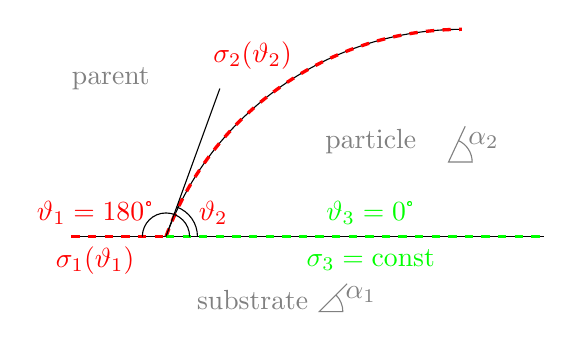
\begin{tikzpicture}
    \draw (-3,0) -- (3,0);
    \draw (-1.8,0) arc (160:90:4);
    \draw[dashed,very thick,red] (-1.8,0) arc (160:90:4);
    \draw[dashed,very thick,red] (-3,0) -- (-1.8,0);
    \draw[dashed,very thick,green] (-1.8,0) -- (3,0);
    
    \draw[gray] (-0.7,-0.8) node {substrate};
    \draw[gray] (0.5,-0.6) -- ++(-135:0.5) -- ++(0.3,0) arc (0:45:0.3) node[right] {$\alpha_1$};
    \draw[gray] (0.8,1.2) node {particle};
    \draw[gray] (2,1.4) -- ++(-115:0.5) -- ++(0.3,0) arc (0:65:0.3) node[right] {$\alpha_2$};
    \draw[gray] (-2.5,2) node {parent};
    
    \draw (-1.8,0) -- +(70:2);
    \draw (-1.8+0.4,0) arc (0:70:0.4);
    \draw[red] (-1.2,0.3) node {$\vartheta_2$};
    \draw[red] (-0.7,2.3) node {$\sigma_2(\vartheta_2)$};
    \draw[red] (-2.7,0.3) node {$\vartheta_1 = 180$\textdegree};
    \draw[red] (-2.7,-0.3) node {$\sigma_1(\vartheta_1)$};
    \draw (-1.8+0.3,0) arc (0:180:0.3);
    
    \draw[green] (0.8,0.3) node {$\vartheta_3=0$\textdegree};
    \draw[green] (0.8,-0.3) node {$\sigma_3=\mathrm{const}$};
\end{tikzpicture}

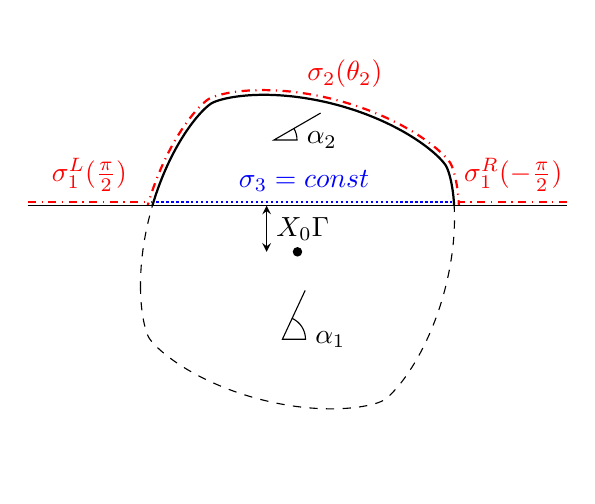
\begin{tikzpicture}[scale=1,font=\normalsize]
    \def\figxwidth{3.5}
    \begin{axis}[
            axis equal,
            disabledatascaling,
            axis line style={draw=none},
            xtick=\empty,
            ytick=\empty,
            xmin=-\figxwidth,xmax=\figxwidth,
            declare function={
                % yshift1=0;
                yshift1=-0.6;
                n=4;
                nsoa=0.9;
                rot1 = 30;
                RW = 0.7*3;
                d=nsoa/(n^2-1);
                aniso1(\t)=1+d*cos(n*(\t-rot1));
                daniso1(\t)=-n*d*sin(n*(\t-rot1));
                Wulffx1(\t) = RW*( aniso1(\t)*cos(\t) - daniso1(\t)*sin(\t) );
                Wulffy1(\t) = RW*( aniso1(\t)*sin(\t) + daniso1(\t)*cos(\t) );
                },
        ]
        \begin{scope}
            \clip (axis cs: -\figxwidth,5) rectangle (axis cs:\figxwidth,0);
            \addplot[domain=-pi:pi, samples=150, smooth, thick] ({Wulffx1(deg(x))},{Wulffy1(deg(x))+yshift1});
            \addplot[domain=-pi:pi, samples=150, smooth, red, dash dot, thick] ({1.03*Wulffx1(deg(x))},{1.03*Wulffy1(deg(x))+yshift1});
        \end{scope}
        
        \begin{scope}
            \clip (axis cs: -\figxwidth,-5) rectangle (axis cs:\figxwidth,0);
            \addplot[domain=-pi:pi, samples=150, smooth,dashed] ({Wulffx1(deg(x))},{Wulffy1(deg(x))+yshift1});
        \end{scope}
        
        \path coordinate (C1) at (axis cs:0,yshift1);
        \path coordinate (B1) at (axis cs:-\figxwidth,0);
        \path coordinate (B2) at (axis cs:\figxwidth,0);
        \path coordinate (zz) at  (axis cs:0,0);
        
        % interfaxce specifications
        \draw (B1) -- (B2);
        \draw[red, dash dot, thick] (axis cs:-\figxwidth,0.05) -- node[midway, above] {$\sigma_{1}^L(\frac{\pi}{2})$} (axis cs:-1.9,0.05);
        \draw[red] (axis cs:0,1.4) node[above right] {$\sigma_{2}(\theta_{2})$} ;
        \draw[red, dash dot, thick] (axis cs:\figxwidth,0.05) -- node[midway, above] {$\sigma_{1}^R(-\frac{\pi}{2})$} (axis cs:2.1,0.05);
        \draw[blue, densely dotted, thick] (axis cs:-1.83,0.05) -- node [midway, above] {$\sigma_{3}=const$} (axis cs:2.0,0.05);
        
        \draw[stealth-stealth] (axis cs:-0.4,0) -- (axis cs:-0.4,yshift1/2) node [right] {$X_0 \Gamma$} -- (axis cs:-0.4,yshift1);
        
        \draw[fill] (C1) circle (1.5pt);
        
        % \draw (axis cs:-2.5,1.5) node [circle,draw,minimum size=6] {$\mathit{3}$};
        % \draw (axis cs:-1,0.8) node [circle,draw,minimum size=6] {$\mathit{2}$};
        % \draw (axis cs:-2.5,-1.5) node [circle,draw,minimum size=6]  {$\mathit{1}$};
        
        % \draw (axis cs: 0,0.8) -- ++(\rtheta{0.5cm}{-150}) -- ++(\rtheta{0.3cm}{0}) node [above right] {l} ;
        \draw (0.3,1.2) -- ++(-150:0.7) -- ++(0:0.3) node [right] {$\alpha_2$} arc (0:30:0.3) ;
        \draw (0.1,-1.1) -- ++(65-180:0.7) -- ++(0:0.3) node [right] {$\alpha_1$} arc (0:65:0.3) ;
    \end{axis}
\end{tikzpicture}


\begin{tikzpicture}[scale=1]
% \def\yline{-0.8};
% \def\xshift{35};
% \def\xline{90-\xshift};
% \def\xxline{90+\xshift};
\def\yline{0.8};
\def\xshift{35};
\def\xline{180-\xshift};
\def\xxline{180+\xshift};
\def\ymin{-1.7};
\def\figw{0.7cm};
\def\insep{0.05cm};
    \begin{axis}[
        xlabel={bottom grain orientation $\alpha_1$ (rad)},
        ylabel={$\cos\left[n(\pi/2-\alpha_1)\right]$ },
        ylabel near ticks,
        xtick = {0},
        extra x ticks = {\xline,\xxline,360},
        extra x tick labels = {,,$\frac{2\pi}{n}$},
        extra y ticks = {\yline},
        extra y tick labels = {$K$},
        legend entries={$n=3$,$n=4$,$n=6$},
        % legend pos = north,
        legend style={legend columns=3,column sep=1ex},
        ymax=1.99,
        ymin=\ymin,
        xmax = 360,
        xmin = -30,
        clip=false
        % ymajorgrids = true
        ]
        
        % \addplot[domain=0:120),samples=50,black] {cos(3*(90-x))};
        % \addplot[domain=0:90),samples=50,red] {cos(4*(90-x))};
        % \addplot[domain=0:60),samples=50,blue] {cos(6*(90-x))};

        % \addplot[domain=0:120),samples=50,black,dashed] {cos(3*(-90-x))};
        % \addplot[domain=0:90),samples=50,red] {cos(4*(-90-x))};
        % \addplot[domain=0:60),samples=50,blue] {cos(6*(-90-x))};
        
        \addplot[domain=0:360,samples=50,black,thick] {-sin(x)};
        \addplot[domain=0:360,samples=50,red,thick] {cos(x)};
        \addplot[domain=0:360,samples=50,blue,thick] {-cos(x)};
        % \addplot[domain=0:360,samples=50,black, dashed] {sin(x)};

        % \draw[dashed, black] (axis cs:-30,\yline) -- (axis cs:\xxline,\yline);
        % \draw[dashed, black,-stealth] (axis cs:\xline,\yline) -- (axis cs:\xline,\ymin);
        % \draw[dashed, black,-stealth] (axis cs:\xxline,\yline) -- (axis cs:\xxline,\ymin);
        % \draw[ black,stealth-stealth] (axis cs:\xline,\ymin-0.08) -- node [midway,below, inner sep = 0.1 cm] {\small unstable} (axis cs:\xxline,\ymin-0.08);

        \draw[dashed, blue] (axis cs:-30,\yline) -- (axis cs:\xxline,\yline);
        \draw[dashed, blue,-stealth] (axis cs:\xline,\yline) -- (axis cs:\xline,\ymin);
        \draw[dashed, blue,-stealth] (axis cs:\xxline,\yline) -- (axis cs:\xxline,\ymin);
        \draw[ blue,stealth-stealth] (axis cs:\xline,\ymin-0.08) -- node [midway,below, inner sep = 0.1 cm] {\small unstable} (axis cs:\xxline,\ymin-0.08);

        \node [above, inner sep=\insep] (w4stab) at (axis cs:0,1) {\includegraphics[width=\figw]{figs/wulff_sketch/sketch_Wulff_4fold_nsoa1-00.pdf}};
        \node [above, inner sep=0*\insep] (w6stab) at (axis cs:180,1) {\includegraphics[width=\figw,angle=30]{figs/wulff_sketch/sketch_Wulff_6fold_nsoa1-00.pdf}};
        \node [above, inner sep=\insep] (w3stab) at (axis cs:270,1) {\includegraphics[width=\figw,angle=90]{figs/wulff_sketch/sketch_Wulff_3fold_nsoa1-00.pdf}};

        \node [below, inner sep=\insep] (w4unstab) at (axis cs:180,-1) {\includegraphics[width=\figw,angle=45]{figs/wulff_sketch/sketch_Wulff_4fold_nsoa1-00.pdf}};
        \node [below, inner sep=2*\insep] (w6unstab) at (axis cs:0,-1) {\includegraphics[width=\figw]{figs/wulff_sketch/sketch_Wulff_6fold_nsoa1-00.pdf}};
        \node [below, inner sep=\insep] (w3unstab) at (axis cs:90,-1) {\includegraphics[width=\figw,angle=30]{figs/wulff_sketch/sketch_Wulff_3fold_nsoa1-00.pdf}};

        \draw[stealth-,thick] (axis cs:270,-1) -- ++(axis direction cs:0,-0.5) -- ++(axis direction cs:20,0)  arc (0:90:20) node [midway, above right, inner sep=0] {$\pi/2$}  ;
        % \draw[stealth-,thick] (axis cs:270,-1) -- ++(axis direction cs:0,-0.4) -- ++(axis direction cs:20,0) node [right] {$\pi/2$} arc (0:90:20) ;
    \end{axis}
\end{tikzpicture}

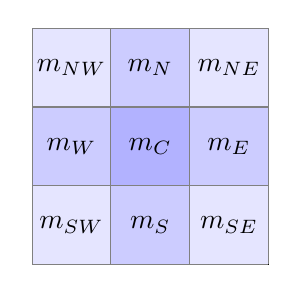
\begin{tikzpicture}
    \draw[fill=blue!10] (0,0) rectangle (3,3);
    \foreach \i/\j in {0/1,1/2,1/1,1/0,2/1}
        \draw[fill=blue!20] (\i,\j) rectangle (\i+1,\j+1);
        
    \draw[fill=blue!30] (1,1) rectangle (2,2);
    
    \draw[gray] (0,0) grid (3,3);
    \draw node at (1.5,1.5) {$m_C$};
    
    \def\colfn{black}
    \draw[\colfn] node at (0.5,1.5) {$m_W$};
    \draw[\colfn] node at (2.5,1.5) {$m_E$};
    \draw[\colfn] node at (1.5,2.5) {$m_N$};
    \draw[\colfn] node at (1.5,0.5) {$m_S$};
    
    \def\colsn{black}
    \draw[\colsn] node at (0.5,0.5) {$m_{SW}$};
    \draw[\colsn] node at (2.5,2.5) {$m_{NE}$};
    \draw[\colsn] node at (0.5,2.5) {$m_{NW}$};
    \draw[\colsn] node at (2.5,0.5) {$m_{SE}$};
\end{tikzpicture}


\begin{tikzpicture}[scale=1]
\def\yline{0.5};
\def\xshift{60};
% \def\yline{0.8};
% \def\xshift{35};
\def\xline{\xshift};
\def\xxline{360-\xshift};
\def\ymin{-1.7};
\def\figw{0.7cm};
\def\insep{0.05cm};
    \begin{axis}[
        xlabel={bottom grain orientation $\alpha_1$ (rad)},
        ylabel={$\cos\left[n(\pi/2-\alpha_1)\right]$ },
        ylabel near ticks,
        xtick = {0},
        extra x ticks = {\xline,\xxline,360},
        extra x tick labels = {,,$\frac{2\pi}{n}$},
        extra y ticks = {\yline},
        extra y tick labels = {$K$},
        legend entries={$n=4$},
        % legend pos = north,
        legend style={legend columns=3,column sep=1ex},
        ymax=1.49,
        ymin=\ymin,
        xmax = 360,
        xmin = -30,
        clip=false
        % ymajorgrids = true
        ]
        
        \addplot[domain=0:360,samples=50,red,thick] {cos(x)};
        % \addplot[domain=\xshift:360-\xshift,samples=50,fill, red!30,thick] {cos(x)} \closedcycle;
        

        \draw[dashed, red] (axis cs:0,\yline) -- (axis cs:\xline,\yline);
        \draw[dashed, red] (axis cs:360,\yline) -- (axis cs:\xxline,\yline);
        \draw[dashed, red,-stealth] (axis cs:\xline,\yline) -- (axis cs:\xline,\ymin);
        \draw[dashed, red,-stealth] (axis cs:\xxline,\yline) -- (axis cs:\xxline,\ymin);
        % \draw[ red,stealth-stealth] (axis cs:0,\ymin-0.08) -- node [midway,below, inner sep = 0.1 cm] {\small unstable} (axis cs:\xline,\ymin-0.08);
        % \draw[ red,stealth-stealth] (axis cs:\xxline,\ymin-0.08) -- node [midway,below, inner sep = 0.1 cm] {\small unstable} (axis cs:360,\ymin-0.08);
        \draw[ red,stealth-stealth] (axis cs:\xline,\ymin-0.08) -- node [midway,below, inner sep = 0.1 cm] {\small stable} (axis cs:\xxline,\ymin-0.08);

        \node [above, inner sep=\insep] (w4stab) at (axis cs:0,1) {\includegraphics[width=\figw]{figs/wulff_sketch/sketch_Wulff_4fold_nsoa1-00.pdf}};

        \node [below, inner sep=\insep] (w4unstab) at (axis cs:180,-1) {\includegraphics[width=\figw,angle=45]{figs/wulff_sketch/sketch_Wulff_4fold_nsoa1-00.pdf}};

        \draw[stealth-,thick] (axis cs:0,-1) -- ++(axis direction cs:0,-0.5) -- ++(axis direction cs:20,0)  arc (0:90:20) node [midway, above right, inner sep=0] {$\pi/2$}  ;
        % \draw[stealth-,thick] (axis cs:270,-1) -- ++(axis direction cs:0,-0.4) -- ++(axis direction cs:20,0) node [right] {$\pi/2$} arc (0:90:20) ;
    \end{axis}

    % \begin{polaraxis}[xshift=3cm,yshift=3cm, width=3cm]
    %     \addplot[]{1};
    % \end{polaraxis}

    \def\nsoa{4} % normalized strength of anisotropy for K=0.5
    \def\angshift{\xshift/4} % half-width of forbidden interval
    % \def\nsoa{2.5} % normalized strength of anisotropy for K=0.8
     % normalized strength of anisotropy
    % \begin{axis}[
    %     xshift=2.9cm,
    %     yshift=3.8cm, 
    %     width=3.8cm,
    %     ymin = 0, ymax = 1.5,
    %     xmin=0, xmax = 1.5,
    %     axis equal image,
    %     ticklabel style={font = \small},
    %     ]
    %     \addplot[data cs = polar, domain=0:90] (x,{1+\nsoa/15*cos(4*x))});
    %     \addplot[data cs = polar, domain=\angshift:(90-\angshift), fill] coordinates {(0,0) (x,{1+\nsoa/15*cos(4*x))}) (0,0) };
        
    % \end{axis}
    \begin{polaraxis}[
        xshift=2.9cm,
        yshift=3.8cm, 
        width=4.2cm,
        ymin = 0, ymax = 1.7,
        xmin=0, xmax = 90,
        axis x line = none,
        ticklabel style={font = \small},
        yticklabel style={yshift=-0.2ex, anchor= east, rotate=60},
        clip=false
        ]
        \addplot[domain=\angshift:(90-\angshift), fill, red!30] (x,{1+\nsoa/15*cos(4*x))}) -- (0,0);
        \addplot[domain=0:90] (x,{1+\nsoa/15*cos(4*x))});
        
        \node[above right,inner sep = 0] at (axis cs: 80,1.5) {\small $f(\theta)/\sigma_0$};
    \end{polaraxis}
\end{tikzpicture}

    
\end{document}
